\documentclass[dvisvgm,multi=true]{standalone}
\usepackage{mathmlcoresvg}
\begin{document}
%<figcaption><span>Figure 18: </span>Box model for the <code>updiagonalstrike</code>
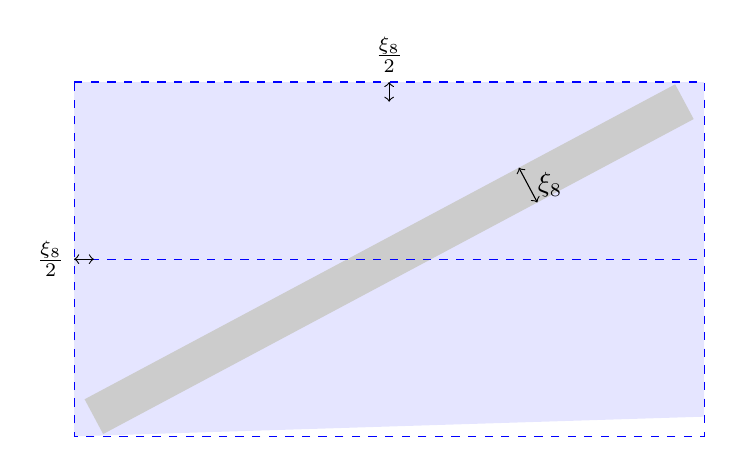
\begin{tikzpicture}[yscale=-1]
  \fill[blue!10]
     (-.25,-2.25) -- (7.75,-2.25) -- (7.75,2) -- (-.25,2.25) -- cycle;
  \MathMLBox{0}{0}{1.5}{1}{red};
  \begin{scope}[shift=({3.75,0}),rotate=-28.07248693585295]
  \fill[black!20] (-4.25,-.25) -- (4.25,-.25) --
                    (4.25,.25) -- (-4.25,.25) -- cycle;
  \draw[<->] (2,-.25) -- (2,0) node[right]{$\xi_8$} -- (2,.25);
  \end{scope}
  \draw[dashed,blue](-.25,-2.25) -- (7.75,-2.25) -- (7.75,2.25) -- (-.25,2.25)
  -- cycle (-.25,0) -- (7.75,0);

  \draw[<->] (0,0) -- (-.25,0) node[left]{$\frac{\xi_8}{2}$};
  \draw[<->] (3.75,-2) -- (3.75,-2.25) node[above]{$\frac{\xi_8}{2}$};
\end{tikzpicture}

\end{document}
